%!TEX TS-program = xelatex
\documentclass[]{friggeri-cv}
\addbibresource{../publications.bib}

\begin{document}
\header{Alessandro Cosentino}{data engineer}
% In the aside, each new line forces a line break
\begin{aside}
    \begin{figure}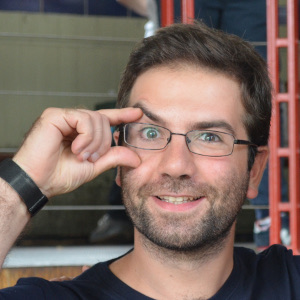
\includegraphics[width=\linewidth]{avatar.jpg}\end{figure}\section{contacts}
    \href{mailto:cosenal@gmail.com}{cosenal@gmail.com}
    \href{https://cosenal.github.io}{https://cosenal.github.io}
  \section{nationality}
    Italian
  \section{languages}
    English
    Italian
\end{aside}

\section{education}
\begin{entrylist}
  \entry
    {2010–2015}
    {Ph.D. {\normalfont in Computer Science}}
    {University of Waterloo}
    {- \emph{Fellow of the Institute for Quantum Computing}\\
     - \emph{Recipient of a David R. Cheriton Graduate Scholarship}}
  \entry
    {2006–2009}
    {M.Math {\normalfont in Computer Science}}
    {University of Pisa}
    {Final score: 110/110 \emph{cum laude}}
  \entry
    {2003–2006}
    {B.Math {\normalfont in Computer Science}}
    {University of Pisa}
    {Final score: 110/110 \emph{cum laude}}
\end{entrylist}

\section{experience}

\begin{entrylist}
  \entry
  {Jan '16–now}
  {Data Engineer}
  {\href{http://www.bendingspoons.com}{Bending Spoons}}
  {Developing an analytical tool for estimating financial data of the mobile apps market through fetching and processing of terabytes of App Store data. }
  \entry
    {2010–2013}
    {Teaching Assistant}
    {University of Waterloo}
    {Courses: Theory of Quantum Information (graduate), Data Structures and Data Management, Algorithms, Introduction to Computer Science.}
  \entry
    {Summer '12}
    {Google Summer of Code Student Developer}
    {KDE}
    {Created the News app, a feed reader for the ownCloud platform.}
  \entry
    {Winter '12}
    {UNIX Consultant}
    {Math Faculty Computing Facility, UWaterloo}
    {Assisted students, faculty and staff with UNIX related problems.}
\end{entrylist}

\section{publications}
\printbibsection{selected}{}
\emph{(This is a selected list of journal publications. For a complete list, see \href{https://scholar.google.com/citations?user=MDj6ntQAAAAJ&hl=en}{Google Scholar})}.
\vspace{5mm}
\section{skills}
\begin{description}
\item[Programming] \emph{Main}: Python ($3+$ yr), MATLAB/Octave ($3$ yr); \emph{Familiar with}: PHP, Javascript; \emph{Prior experience}: OCaml, Go, C++;
\item[Data Engineering] AirFlow, Spark, Redis, PostgreSQL, BigQuery, Re:dash;
\item[Data Analysis] R, pandas, scikit-learn, Excel;
\item[Web] Flask, HTML5, AngularJS framework, CSS;
\item[Other] Heroku toolbox, Git, Bash, RSS and Atom standards, \LaTeX.
\end{description}
\end{document}
